\documentclass[doc, floatsintext]{apa7}
\usepackage[style=apa,sortcites=true,sorting=nyt,backend=biber]{biblatex}
\DeclareLanguageMapping{american}{american-apa}
\addbibresource{citations.bib}
\usepackage{amsmath}
\usepackage{float}
\usepackage{graphicx}
\usepackage{mathrsfs}
\usepackage{setspace}
\setstretch{1.0}
\usepackage{caption}
\usepackage{gensymb}

\title{Motor demands in catogory learning during task switching}

\shorttitle{Category learning during task switching}

\authorsnames[{1, 2}, {1}, {1, 2}, {3}]{
    Matthew J. Crossley, 
    Hannah Arnold, 
    David M. Kaplan, 
    F. Gregory Ashby
}

\authorsaffiliations{
    {School of Psychological Sciences, Macquarie University, Sydney, Australia}, 
    {Macquarie University Performance and Expertise Research Centre, Macquarie University, Sydney, Australia},
    {Department of Psychological \& Brain Sciences, University of California, Santa Barbara}
    }

\authornote{Correspondence: Matthew J. Crossley, PhD,
  School of Psychological Sciences, Macquarie University,
  Australian Hearing Hub, 16 University Ave, Macquarie
  University, NSW 2109, Australia. Email:
  matthew.crossley@mq.edu.au 
}


\keywords{category learning, task switching, Cognitive control}

\begin{document}
\maketitle
\newpage

\section{Abstract}
Procedural category learning involves forming many-to-one
stimulus-response (SR) associations through trial-and-error
feedback. While single-task contexts suggest these
associations are linked to motor goals (e.g., pressing a
button on the left) rather than specific motor effectors
(e.g., pressing with a particular finger), it is unknown if
this holds in task-switching contexts.  In this study, we
investigated whether category learning during task-switching
relies on motor goal-based SR associations or shifts to an
effector-specific level. Participants learned two category
structures while switching tasks from the beginning of
training. Our results revealed that learning was more
effective when stimuli from a specific region of stimulus
space were mapped to different fingers on the same hand, as
opposed to different fingers on opposite hands. Nonetheless,
significant learning occurred in both cases. These findings
suggest that procedural category learning during task
switching involves forming SR associations tied to both
motor goals and, to some extent, motor effectors.

\section{Introduction}
In task-switching experiments, participants are asked to
perform two distinct tasks in a pseudo-random interleaved
order \parencite{kiesel_control_2010, monsell_task_2003}.
Most studies have focused on switching between well-learned
tasks that can be performed with high accuracy in isolation.
Little attention has been given to how task switching
operates when tasks must be learned simultaneously.

We are aware of only two lines of research that have begun
to explore simultaneous learning of new tasks during task
switching.  First, Collins and colleagues have studied
simple tasks with highly discernible stimuli and
straightforward response rules
\parencite{collins_cognitive_2013, collins_human_2014,
collins_neural_2016, collins_motor_2016, collins_cost_2017}.
These tasks, due to their simplicity, are rapidly learned,
limiting the scope for investigating how task switching
interacts with the learning process itself. Moreover, these
tasks rely heavily on declarative memory and explicit
reasoning. The question of how task switching impacts
procedural learning remains largely unexplored.

Our lab has begun to address this gap by examining task
switching with more complex, procedural category learning
tasks that do not lend themselves to rapid learning
\parencite{crossley_switch_2023,
crossley_trial-by-trial_2018, turner_hierarchical_2017}. A
key finding from this research is that learning under task
switching is only reliably successful when the motor
responses for each task are distinct
\parencite{crossley_switch_2023}. 

Procedural category learning involves forming
stimulus-response (SR) associations through trial-and-error
feedback. Ashby, Ell, and Waldron (2003) provided key
evidence for procedural learning in certain categorization
tasks. They showed that performance was unaffected by
switching hands but was impaired by switching key locations,
suggesting that SR associations are linked to motor goals
(e.g., pressing a key on the left) rather than motor
effectors (e.g., pressing with a specific finger).

While this suggests that the SR associations in single-task
contexts operate at the motor goal level, it remains unclear
whether this holds while task switching. In this study, we
investigated whether procedural category learning during
task switching occurs at the level of motor goals or whether
it occurs at the level of motor effectors.

\section{Methods}

\subsection{Design}
We examined category learning while participants switched on
a random trial-by-trial basis between two different
categorization tasks.   Each task was an
information-integration (II) category-learning task, in
which the optimal strategy is similarity based, and for
which no simple verbal rule
\parencite{ashby_neuropsychological_1998,
ashby_decision_1988} can achieve perfect accuracy.   On
every trial in both tasks, the participant was instructed to
assign the single presented stimulus to its correct
category.  The stimuli in both tasks were circular sine-wave
gratings that varied across trials in their spatial
frequency and their orientation.   Gratings in the first
task were presented on a gray square background on top of a
black screen, whereas gratings in the second task were
presented on a gray diamond background on top of a black
screen. See Figure~\ref{fig_example_trials.png} for
examples.

\begin{figure}[h!]
    \centering
    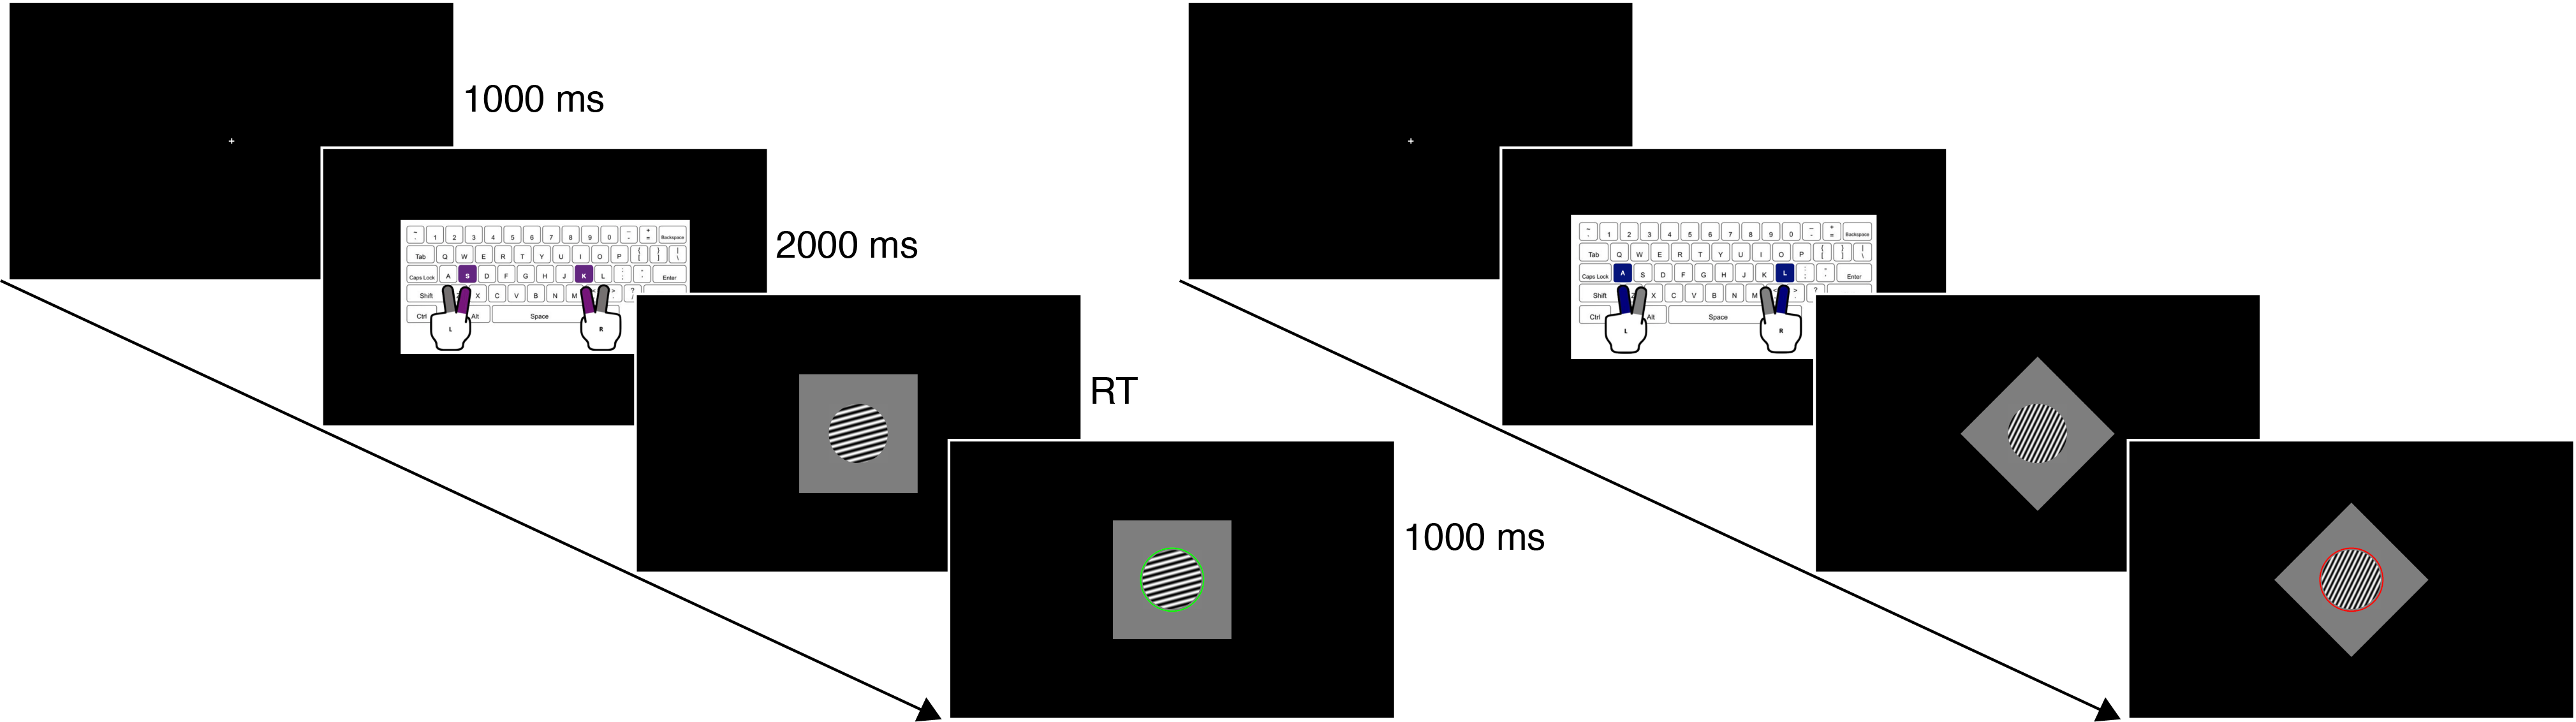
\includegraphics[width=\textwidth]{../figures/fig_example_trials.png}
    \caption{
    \textbf{Left:} Example Square subtask trial in which a
    correct response was given.  \textbf{Right:} Example
    Diamond subtask trial in which an incorrect response was
    given.
}
    \label{fig_example_trials.png}
\end{figure}

Subjects were randomly assigned to one of two conditions --
Congruent or Incongruent.  The
Congruent is named to reflect the nature of how
stimuli were assigned to specific fingers. In particular,
stimuli from different tasks but from the same regions of
stimulus space were assigned to fingers on the same hand.
In the Incongruent condition, participants were
required to use the same set of keys as in the
Congruent condition.  However stimuli from
different tasks but from the same regions of stimulus space
were to fingers on different hands.  This is the sense in
which the Congruent condition is congruent and the
Incongruent condition is incongruent.  Please see
Figure~\ref{fig_example_trials.png} for an illustration
of the exact mappings used.

\subsection{Participants}
We recruited 91 participants to serve as participants.   One
participant was excluded from the analysis for failing to
follow the instructions regarding which fingers and keys to
use to indicate category responses. The remaining 90
participants were either first-year undergraduate psychology
students from Macquarie University recruited via the Sona
system ($n = 28$) or individuals from the general community
($n = 62$), recruited via direct invitation from the
researchers. All Macquarie University undergraduate
participants completed the study and received course credit
for their participation.  All other participants volunteered
with no compensation. All participants were between 18 to 30
years of age, fluent in English, had normal or
corrected-to-normal vision and hearing and no history of
neurological impairments. Each participant was randomly
assigned to one of 2 conditions (named Congruent and
Incongruent).  Of the 45 incongruent participants there were
12 males and 31 females. Their ages ranged from 18 to 27
years old ($M = 19.6$, $SD = 1.7$).  Of the 45 congruent
participants there were 16 males and 29 females. Their ages
ranged from 18 to 30 years old ($M = 22.5$, $SD = 2.3$).  

\subsection{Stimuli and Categories}
The stimuli were circular sine wave gratings that varied in
spatial frequency and orientation.  Stimuli coordinates were
generated by first sampling points in polar coordinates and
then converting them into Cartesian coordinates.
Specifically, a radius values $r$ were sampled from a
uniform distribution on the interval $[0, 1]$, and angle
values $\theta$ were sampled uniformly on $[0, 2\pi]$.
These polar coordinates $(r, \theta)$ were then transformed
into Cartesian coordinates $(x, y)$ using the equations $x =
r \cos(\theta)$ and $y = r\sin(\theta)$. This resulted in a
set of $(x, y)$ coordinates uniformly distributed within a
circle of radius 1 and centered at the origin. Next, $(x,
y)$ coordinates were transformed from a circular uniform
distribution to an elliptical uniform distribution with it's
major axis along the horizontal axis by multiplying the $x$
values by 124.02 and the $y$ values by 28.44. Finally, the
resulting coordinates were rotated by 45\degree and
translated by $(40, 60)$ for half the stimuli and by $(60,
40)$ for the other half. The resulting stimuli distributions
are shown in Figure~\ref{fig_categories_stim_space.png}.

\begin{figure}[h!]
    \centering
    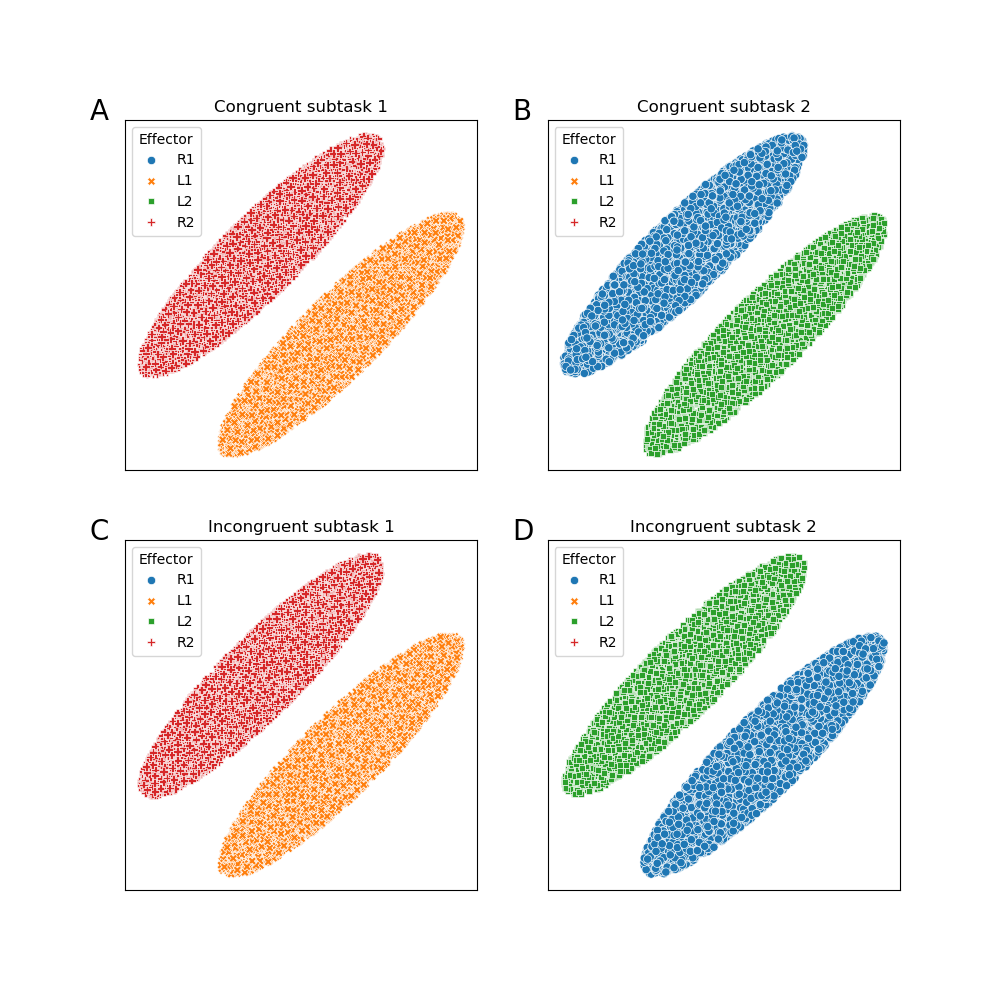
\includegraphics[width=0.7\textwidth]{../figures/fig_categories_stim_space.png}
    \caption{
        \textbf{A:} Stimuli distributions for the Square task in the Congruent condition.
        \textbf{B:} Stimuli distributions for the Diamond task in the Congruent condition.
        \textbf{C:} Stimuli distributions for the Square task in the Incongruent condition.
        \textbf{D:} Stimuli distributions for the Diamond task in the Incongruent condition.
        In all panels, the colour of the points indicates
        the effector -- and thus the response key -- that
        indicates the correct category for that stimulus. R1
        stands for the right index finger, R2 for the right
        middle finger, L1 for the left index finger, and L2
        for the left middle finger. The key feature of the
        Incongruent condition is that stimuli from the same
        region of stimulus space are assigned to different
        hands in different subtasks.
    }
    \label{fig_2}
\end{figure}

\subsection{Procedure}
Participants were first given a paper information and
consent form and were required to sign and date the form
before proceeding. They were also given an optional
demographic questionnaire to complete. Participants were
then given verbal instructions with the aid of slides (see
the Appendix). Briefly  participants in all conditions were
told that they were to categorize circular sine wave
gratings on the basis of their spatial frequency and
orientation, and that each category was equally likely.
They were also instructed that gratings presented on a
square background may or may not require a different
response policy than gratings presented on a diamond
background. 

% TODO: check trial timing reported below
Each participant completed a single session consisting of
400 trials, with each task (square or diamond) interleaved
psuedo-randomly.   On each trial, participants viewed a
fixation cross (1000 ms), followed by a cue image that
indicated the correct finger-key mapping for the upcoming
task (2000 ms), followed by a response-terminated stimulus,
and then feedback (1000 ms).  Responses were given via the
``a'', ``s'', ``k'' and ``l'' keys as indicated by the cue
image (see Figure~\ref{fig_example_trials}. Feedback
following correct responses was a green circle that appeared
around the stimulus, and feedback following incorrect
responses was a red circle. See
Figure~\ref{fig_example_trials.png} an illustration of
example trials.

\subsection{Statistical Analysis}
We performed a logistic regression to examine learning as a
function of condition (Congruent vs Incongruent),
best-fitting decision-bound model (rule-based vs
procedural), and log trial. All categorical predictors
(i.e., condition and best-fitting decision-bound model) were
dummy coded. Log trial number was used rather than trial
number to account for the fact that the learning apparent in
Figure~\ref{fig_learning_curves} is non-linear, with more
rapid initial improvements followed by slowed improvements
as the task progresses. To assess whether there were
differences in the proportion of participants best fit by a
rule-based or procedural decision-bound model in each
condition, we conducted a $\chi^2$ test. To assess switch
costs, we computed the difference in accuracy and RT between
switch trials and stay trials for all trials across the
entire experiment for each participant. We then conducted a
2 (condition) x 2 (best-fitting decision-bound model) ANOVA
on the resulting switch costs.

\subsection{Decision-Bound Analysis}
To identify the decision strategy used by each participant,
we fit decision-bound models
\parencite{maddox_comparing_1993, ashby_decision_1988} to
the trial-by-trial response data from the final 100 trials
of the experiment separately for each subtask. We examined
1-dimensional rule-based models and 2-dimensional procedural
models.  The rule-based models assumed participants
established a criterion on a single stimulus dimension and
then categorized stimuli based on whether they exceeded this
criterion. These models had two free parameters. One
parameter that determined the criterion value and a second
parameter that determined the variance of perceptual and
criterial noise. The 2-dimensional procedural models --
i.e., general linear classifier (GLC) --  assumed that
participants used a linear decision boundary with an
arbitrary slope and intercept.  Stimuli were categorized
based on their position relative to this boundary. The GLC
has three free parameters. One parameter that determined the
slope of the boundary, a second parameter that determined
the intercept of the boundary, and a third parameter that
determined the variance of perceptual and criterial noise.
For details, see \textcite{ashby_multiple_2017}.

\section{Results}

\subsection{Learning Curves}
Figure~\ref{fig_learning_curves}A shows the mean accuracy
per trial averaged over all participants for each condition.
The semi-transparent lines show performance separately for
each subtask and the solid lines show performance averaged
over both subtasks.  This figure clearly indicates that
learning proceeded more quickly and to a larger extent in
the Congruent condition than in the Incongruent condition.
Figure~\ref{fig_learning_curves}B shows the results for
participants best fit by a rule-based decision-bound model
and Figure~\ref{fig_learning_curves}C shows the results for
participants best fit by a procedural decision-bound model
(see the ``Decision Bound Models'' section for details). The
trend in both of these panels is the same as that observed
when considering all participants regardless of best-fitting
model (Figure~\ref{fig_learning_curves}A).

\begin{figure}[h!]
    \centering
    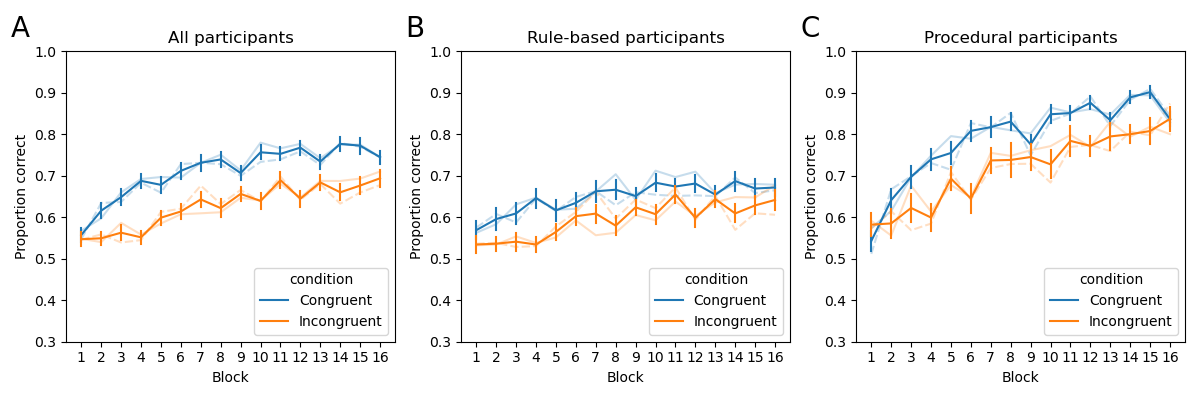
\includegraphics[width=0.8\textwidth]{../figures/fig_accuracy_per_block_by_model.png}
    \caption{
        \textbf{A:} Mean accuracy per block in averaged over
        all participants. \textbf{B:} Mean accuracy per block
        in averaged over participants best fit by a
        rule-based decision-bound model.  \textbf{C:} Mean
        accuracy per block in averaged over participants
        best fit by a procedural decision-bound model.
        In all panels, blue lines correspond to the
        Congruent condition and orange lines correspond to
        the Incongruent condition.  The semi-transparent
        lines show the performance in each subtask, and the
        solid lines show the performance averaged over both
        subtasks. Error bars are standard errors of the
        mean.
    }
    \label{fig_learning_curves}
\end{figure}

We conducted a logistic regression to examine the effects of
experimental condition (Congruent vs.  Incongruent),
decision-bound model (DBM: rule-based vs.  procedural), and
their interactions on accuracy.  The results are summarized
in Table \ref{tab_logistic_regression}.  See the
``Statistical Analysis'' section for details. 
%
The effect of $\log(\text{trial})$ was significant ($\beta =
0.4775$, SE = 0.026, $z = 18.211$, $p < .001$), indicating
that accuracy increased across trials.  
%
The effect of Condition was not statistically significant
($\beta = 0.2289$, SE = 0.205, $z = 1.119$, $p = .263$),
indicating that overall accuracy in the Congruent and
Incongruent conditions was similar. 
%
However, the interaction between Condition and
$\log(\text{trial})$ was significant ($\beta = -0.1321$, SE
= 0.041, $z = -3.205$, $p = .001$), indicating that accuracy
improved across trialsl more rapidly for the Congruent
condition than in the Incongruent condition.
%
The three-way interaction of Condition, best-fitting
decision-bound, and $\log(\text{trial})$ was also
significant ($\beta = 0.1361$, SE = 0.050, $z = 2.735$, $p =
.006$), indicating that the rate of improvement in accuracy
across trials was greater in the Congruent condition than in
the Incongruent condition but only for participants best fit
by a procedural model.
%
Overall accuracy was also significantly greater for
participants best fit by a procedural model than for
participants best fit by a rule-based model ($\beta =
0.9020$, SE = 0.167, $z = 5.386$, $p < .001$)
%
Participants best fit by a procedural model also showed a
greater improvement in accuracy across trials than
participants best fit by a rule-based model ($\beta =
-0.3348$, SE = 0.034, $z = -9.937$, $p < .001$).
%
The interaction between Condition and best fitting
decision-bound model was not significant ($\beta = -0.4712$,
SE = 0.249, $z = -1.895$, $p = .058$).

\begin{table}
\begin{center}
\begin{tabular}{lcccccc}
                                              & \textbf{coef} & \textbf{std err} & \textbf{z} & \textbf{P$> |$z$|$} & \textbf{[0.025} & \textbf{0.975]}  \\
\midrule
\textbf{Intercept}                            &      -1.0034  &        0.129     &    -7.796  &         0.000        &       -1.256    &       -0.751     \\
\textbf{Condition}                            &       0.2289  &        0.205     &     1.119  &         0.263        &       -0.172    &        0.630     \\
\textbf{DBM}                                  &       0.9020  &        0.167     &     5.386  &         0.000        &        0.574    &        1.230     \\
\textbf{Condition:DBM}                        &      -0.4712  &        0.249     &    -1.895  &         0.058        &       -0.959    &        0.016     \\
\textbf{log(trial)}                           &       0.4775  &        0.026     &    18.211  &         0.000        &        0.426    &        0.529     \\
\textbf{condition:log(trial)}                 &      -0.1321  &        0.041     &    -3.205  &         0.001        &       -0.213    &       -0.051     \\
\textbf{DBM:log(trial)}                       &      -0.3348  &        0.034     &    -9.937  &         0.000        &       -0.401    &       -0.269     \\
\textbf{Condition:DBM:log(trial)}             &       0.1361  &        0.050     &     2.735  &         0.006        &        0.039    &        0.234     \\
\bottomrule
\end{tabular}
\label{tab_logistic_regression}
\end{center}
\caption{Logistic regression results. Condition is dummy
    coded with the Incongruent condition as the reference.
    Decidion-bound model (DBM) is dummy coded with the
    rule-based model as the reference.
}
\end{table}

\subsection{Task Switching}
Figure~\ref{fig_switch_cost} shows switch costs for for
accuracy and RT for Congruent and Incongruent conditions for
all participants, participants best fit by a rule-based
decision-bound model, and participants best fit by a
procedural decision-bound. A 2 (condition) x 2 (best-fitting
decision-bound model) ANOVA revealed that the effect of
condition was significant ($F(1, 86) = 8.74, p < .001,
\eta^2 = 0.09$), indicating that switch costs were greater
in the Incongruent condition than in the Congruent condition
(see Figure \ref{fig_switch_cost}). However, the difference
in switch cost between participants best fit by a procedural
model and participants best fit by a rule-based model was
not significant $F(1, 86) = 0.02, p = .88, \eta^2 = 0.00$.
The interaction term was also non-significant, $F(1, 86) =
0.01, p = .93, \eta^2 = 0.00$. 

\begin{figure}[h!]
    \centering
    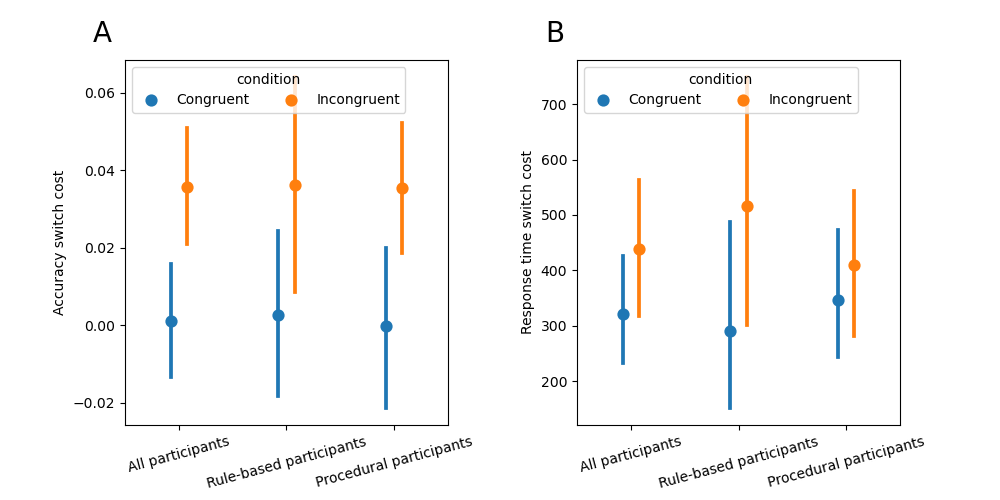
\includegraphics[width=0.7\textwidth]{../figures/fig_switch_cost.png}
    \caption{
        Accuracy switch costs \textbf{A} and RT switch costs
        \textbf{B} for both Congruent (blue) and Incongruent
        (orange) conditions for all participants,
        participants best fit by a rule-based decision-bound
        model, and participants best fit by a procedural
        decision-bound model.
    }
    \label{fig_switch_cost}
\end{figure}

\subsection{Decision Bound Models}
Figure~\ref{fig_dbm.pdf} panels A, B, D, and E show the
decision bounds from the best-fitting decision-bound models
in both conditions overlaid on the underlying category
distribution for each subtask.  Figure~\ref{fig_dbm.pdf}
panels C and F show the proportion of participants whose
responses were best fit by each type of model in each
condition. For this analysis, we coded each particpant as a
procedrual model user if they were best by a GLC model on
both subtasks, or as a rule-based model user if they were
best fit by a RB model on either subtask. This figure
clearly shows that there were more procedural users in the
Congruent condition than in the Incongruent condition.  The
results of Pearson's Chi-Squared test revealed that there
were signifcantly more participants best fit by a procedural
model in the Congruent condition than in the Incongruent
condition ($\chi^2(1, N = 200) = 4.48, p = .034,
\text{Cramer’s} V = 0.16$).

\begin{figure}[h!]
    \centering
    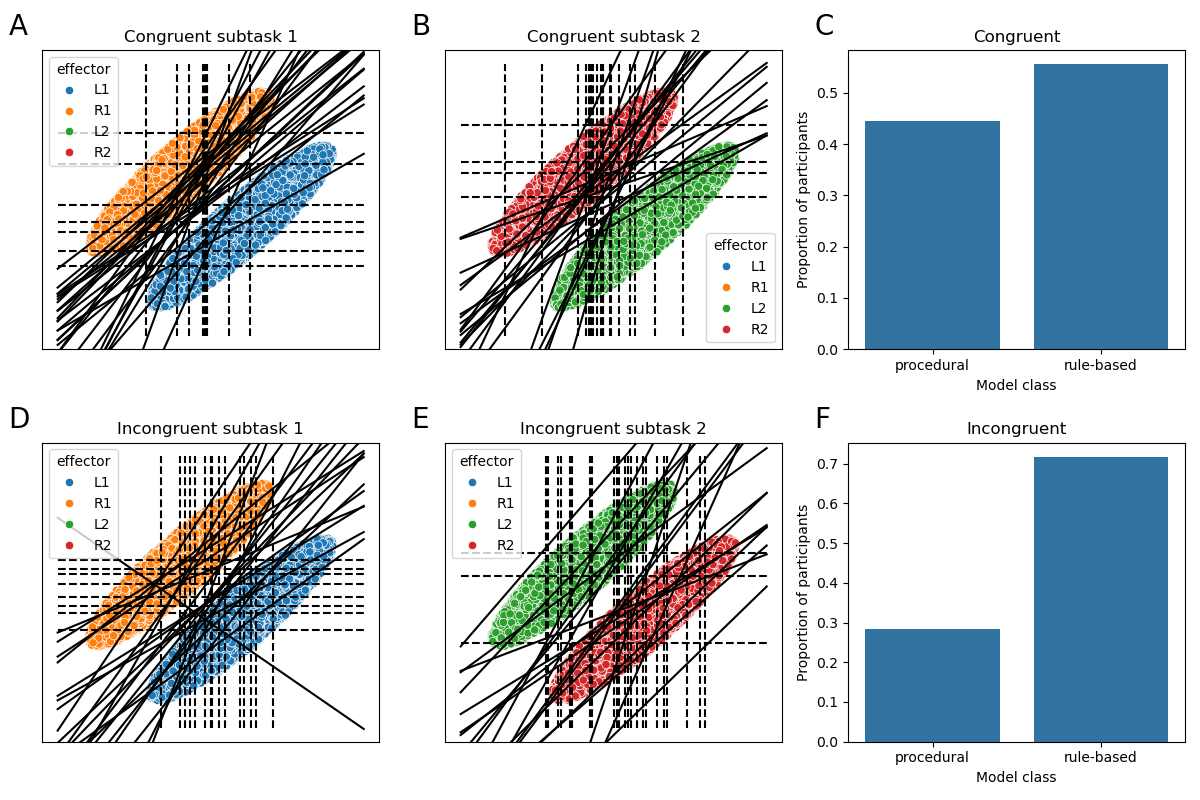
\includegraphics[width=0.7\textwidth]{../figures/fig_dbm.png}
    \caption{
        Category structures and decision bounds from the
        best-fitting decision bound model for each participant
        and subtask in each condition during the final 100
        trials of training. 
        \text{A:} Decision bounds for the Square task in the Congruent condition.
        \text{B:} Decision bounds for the Diamond task in the Congruent condition.
        \text{C:} Proportion of participants best fit by a procedural model in each condition.
        \text{D:} Decision bounds for the Square task in the Incongruent condition.
        \text{E:} Decision bounds for the Diamond task in the Incongruent condition.
        \text{F:} Proportion of participants best fit by a procedural model in each condition.
    }
    \label{fig_dbm}
\end{figure}

\section{Discussion}
Procedural category learning involves the gradual formation
of many-to-one stimulus-response (SR) associations through
trial-and-error feedback. Previous research in single-task
contexts suggests that these associations are linked to
motor goals (e.g., pressing a button on the left) rather
than specific motor effectors (e.g., pressing a button with
a particular finger). The current study aimed to extend this
finding to task-switching contexts, investigating whether SR
associations remain goal-based or shift to an
effector-specific level when tasks are switched.
Participants learned two category structures while switching
between tasks from the start of training, with motor
responses varying across tasks. Our results showed more
effective learning when stimuli from the same region of
stimulus space were mapped to responses on the same hand
(Congruent condition), compared to when different hands were
used (Incongruent condition). These findings suggest that
procedural category learning continues to rely primarily on
motor goal-based SR associations during task switching.
However, the fact that learning also occurred in the
Incongruent condition indicates that effector-specific
associations may also play a role.

\subsection{Context cues and response generalization}
A more refined interpretation of our results can be gleaned
by considering  how participants used (or failed to use) the
context cue meant to differentiate between the two tasks.
There are three main possibilities: (1) the context cue was
used perfectly, enabling participants to form independent,
context-specific SR associations; (2) the context cue was
entirely ignored; or (3) it was used imperfectly, leading to
some degree of generalization or interference between
contexts. 

First, if participants had successfully formed independent
SR associations for each task, we would expect no difference
in learning performance between the Congruent and
Incongruent conditions. Each task would have been learned in
isolation, with no interference or generalization across
contexts. However, given the significant difference in
learning outcomes between the two conditions, this
explanation is inconsistent with our findings. Second, if
participants entirely ignored the context cue, there would
be no cost associated with switching between contexts. Yet,
our data show clear switch costs in both conditions, making
it unlikely that participants disregarded the context cue,
and thus, we can rule out this possibility. Third, if
participants did form separate SR associations for each task
but these associations were subject to some degree of
generalization or interference across contexts, several
possibilities emerge.

If learning and generalization occurred at the motor goal
level rather than the effector level, we would expect strong
learning in the Congruent condition. This is because stimuli
from the same region of stimulus space would consistently be
associated with the same motor goal (e.g., pressing a
left-hand button) across both tasks. Learning in the
Incongruent condition, however, would be impaired relative
to the Congruent condition -- depending on the extent of
generalization between contexts -- because stimuli from the
same region of stimulus space would be associated with
different motor goals in each task. This possibility aligns
well with our findings.

If learning and generalization occurred at the effector
level, the degree of generalization between effectors would
dictate learning outcomes. Without any generalization,
learning would fail in both conditions. This is because
stimuli from the same region of stimulus space would require
different motor responses across tasks.  However, if
generalization occurred between fingers on the same hand,
learning could still succeed in the Congruent condition but
not in the Incongruent condition. If generalization extended
to mirrored fingers on opposite hands, learning would also
occur in the Incongruent condition. Thus, our results
suggest that there may be a higher degree of generalization
between fingers on the same hand and, to a lesser extent,
between mirrored fingers on opposite hands.

In summary, our findings imply that if the response
component of the SR associations driving procedural category
learning operate at the motor goal level, there is some
degree of generalization between contexts such that the goal
associations learned in one context can be used or must be
overcome in another context. Conversely, if the response
component operates at the effector level, our results
suggest greater generalization occurs between fingers on the
same hand than between mirrored fingers on opposite hands.
This interpretation broadly aligns with anatomical evidence
showing that finger representations in M1 -- while
somatotopic -- widey overlap for neighboring fingers (REFS).

% 23. Dechent P, Frahm J. Functional somatotopy of finger
% representations in human primary motor cortex. Hum Brain
% Mapp 2003; 18:272–83. PMID: 12632465
% 
% 24. Ejaz N, Hamada M, Diedrichsen J. Hand use predicts the
% structure of representations in sensorimotor cortex. Nat
% Neurosci 2015;18.
% 
% 25. d’Avella A, Giese M, Ivanenko YP, Schack T, Flash T.
% Editorial: Modularity in motor control: from muscle
% synergies to cognitive action representation. Front Comput
% Neurosci 2015; 9:1–6.
% 
% 26. d’Avella A, Saltiel P, Bizzi E. Combinations of muscle
% synergies

\subsection{Relation to existing lines of research}
This study builds upon our previous investigation into the
effects of motor planning on task-switching in novel and
attention-demanding tasks \parencite{crossley_switch_2023,
crossley_trial-by-trial_2018, turner_hierarchical_2017}.  In
that earlier work, we were among the first to explore task
switching when the tasks are not only new to participants
but also challenging to learn.  One of the key findings was
that learning while task-switching was only possibly when
each task involved unique motor responses.  In the present
study, we extend this line of inquiry by showing that the
stimulus-response (SR) associations formed during task
switching are primarily at the motor goal level, but also at
the effector level. 

A line of studies from Collins and colleagues is also
relevant to our current results
\parencite{collins_cognitive_2013, collins_human_2014,
collins_neural_2016, collins_motor_2016, collins_cost_2017}.
In particular \textcite{collins_motor_2016} showed that when
task switching, humans prefer hierarchical rules in which
the motor responses used for within a task are adjacent.
However, it is not simple to connect our results to theirs
since their studies used relatively simple tasks
characterized by easily discernible stimuli and
straightforward response rules, whereas ours was difficult
to learning and relied on procedural learning.

% TODO: write conclusion
\subsection{Conclusions}
Put smart and important sounding stuff here.

\subsection{Authors' contributions}
MJC wrote the paper, designed the experiments, performed all data analysis and modelling, and and oversaw data collection;
HA wrote the paper and collected all data.
DMK wrote the paper and oversaw data collection;
FGA wrote the paper and designed the experiments.

\printbibliography

\end{document}
